\documentclass[12pt]{article} 
\usepackage[utf8]{inputenc}
\usepackage{geometry}
\geometry{letterpaper}
\usepackage{graphicx} 
\usepackage{parskip}
\usepackage{booktabs}
\usepackage{array} 
\usepackage{paralist} 
\usepackage{verbatim}
\usepackage{subfig}
\usepackage{fancyhdr}
\usepackage{sectsty}
\usepackage{xcolor}

\pagestyle{fancy}
\renewcommand{\headrulewidth}{0pt} 
\lhead{}\chead{}\rhead{}
\lfoot{}\cfoot{\thepage}\rfoot{}

%%% SECTION TITLE APPEARANCE
\allsectionsfont{\sffamily\mdseries\upshape} 

%%% ToC (table of contents) APPEARANCE
\usepackage[nottoc,notlof,notlot]{tocbibind} 
\usepackage[titles,subfigure]{tocloft}
\renewcommand{\cftsecfont}{\rmfamily\mdseries\upshape}
\renewcommand{\cftsecpagefont}{\rmfamily\mdseries\upshape} %

\usepackage{amsmath}
\usepackage{amssymb}
\usepackage{empheq}

\renewcommand{\L}[1]{\mathcal{L}\{#1\}}
\newcommand{\ans}[1]{\boxed{\text{#1}}}
\newcommand{\brak}[1]{\langle#1\rangle} 

\title{Homework 2}
\author{Milan Capoor}
\date{10 February 2023}

\begin{document}
\maketitle
\textbf{Problem 1:} Solve 
\[\begin{cases}
    (1 + x^2)u_x + u_y = 0\\
    u(0, y) = y^3
\end{cases}\]

\color{blue}
Using the directional derivative:
\[(1 + x^2)u_x + u_y = \nabla u \cdot \brak{1 +x^2, 1}\]
So $u$ is constant along curves with "slope" $\frac{1}{1+x^2}$
Taking the characteristic lines:
\[y'(x) = \frac{1}{1+x^2}\]
\[y = \tan^{-1} x + C \implies y - \tan^{-1} x = C\]
\[u(x, y) = f(y - \tan^{-1} x)\]
Initial condition:
\[u(0, y) = y^3 = f(y - \tan^{-1} 0) = f(y) \implies f = y^3\]
\[\ans{$u(x, y) = (y - \tan^{-1}x)^3$}\]
\color{black}

\pagebreak
\textbf{Problem 2:} Solve $u_x + u_y = 1$ \footnote{
    Note: Just like for linear ODE, it is enough to find the general solution of $u_x + u_y = 0$ and one particular solution to $u_x + u_y = 1$ (which you can guess) and add the two together}

\color{blue}
Homogeneous solution:
\[u_x + u_y = 0 \implies \nabla u \cdot \brak{1, 1}\] 
\[\frac{1}{1} = y' \implies m = 1 \implies y = x + C\]
\[y - x = C\]
\[u(x, y) = f(y - x)\]

Particular solution:
\[g(x, y) = x\]
\[g_x + g_y = 1 + 0 = 1 \checkmark\]

General solution:
\[\ans{$u(x, y) = f(y - x) + x$}\]
\color{black}

\pagebreak
\textbf{Problem 3:} Solve $au_x + bu_y + cu =0$ where $a, b, c$ are constants and $a \neq 0$ \footnote{
    Hint: Let $v(x, y) = u(x, y)e^{\frac{cx}{a}}$ and find a PDE for v. For this, solve for u in terms of v and calculate $u_x$ and $u_y$

    Note: if you're completely stuck, check out: Transform method}

\color{blue}
    Note that 
    \[u_x + \frac{c}{a}u = -\frac{b}{a}u_y\]
    Which by ODE integrating factors is
    \[\left(ue^{\frac{cx}{a}}\right)_x = -\frac{b}{a}u_ye^{\frac{cx}{a}}\]
    Let $v(x, y) = u(x, y)e^{\frac{cx}{a}}$ giving 
    \[v_x = -\frac{b}{a}u_ye^{\frac{cx}{a}}\]
    \[v_x = -\frac{b}{a}v_y\]
    \[av_x + bv_y = 0\]
    \[v(x, y) = f(ay - bx)\]

    But because we already know v:
    \[v(x, y) = f(ay - bx) = u(x, y)e^\frac{cx}{a}\]
    
    Thus, rearranging 
    \[\ans{$u(x,y) = e^{-\frac{cx}{a}}f(ay - bx)$}\]
    
    Checking:
    \begin{align*}
        u_x &= -\frac{c}{a}e^{-\frac{cx}{a}}f(ay - bx) - be^{-\frac{cx}{a}}f'(ay - bx)\\
        u_y &= ae^{-\frac{cx}{a}}f'(ay - bx)\\
    \end{align*}
    \[au_x + bu_y + cu = 0\]
    \[-ce^{-\frac{cx}{a}}f(ay - bx) - abe^{-\frac{cx}{a}}f'(ay - bx) + abe^{-\frac{cx}{a}}f'(ay - bx) + ce^{-\frac{cx}{a}}f(ay - bx) = 0\]
    \[-abe^{-\frac{cx}{a}}f'(ay - bx) + abe^{-\frac{cx}{a}}f'(ay - bx) = 0 = 0 \quad \checkmark\]

\color{black}

\pagebreak 
\textbf{Problem 4:} Use the coordinate method to solve \footnote{
    Hint: One of the coordinates is in the equation, for the other one, think perpendicular
}
\[u_x + 2u_y + (2x-y)u = 0\]

\color{blue}
\[\begin{cases}
    x' = x + 2y\\
    y' = -2x + y
\end{cases}\]

Chain rule:
\begin{align*}
    u_x &= \frac{\partial u}{\partial x'}\frac{\partial x'}{\partial x} + \frac{\partial u}{\partial y'}\frac{\partial y'}{\partial x} = u_{x'} - 2u_{y'}\\
    u_y &= \frac{\partial u}{\partial x'}\frac{\partial x'}{\partial y} + \frac{\partial u}{\partial y'}\frac{\partial y'}{\partial y} = 2u_{x'} + u_{y'}
\end{align*}

Substituting,
\[u_x + 2u_y + (2x-y)u = 0\]
\[(u_{x'} - 2u_{y'}) + 2(2u_{x'} + u_{y'}) + (2x-y)u = 0\]
\[5u_{x'} + (2x-y)u = 0\]

Solving via ODE:
\[u_{x'} + \frac{1}{5}(2x-y)u = 0\]
\[(ue^{\int \frac{2x - y}{5} \; dx'})_{x'} = 0\]
\[(ue^{-\frac{1}{5}\int y' \; dx'})_{x'} = 0\]
\[ue^{-\frac{1}{5}y'x'} = f(y')\]
\[u = e^{\frac{1}{5}y'x'}f(y')\]
\[\ans{$u(x, y) = e^{\frac{1}{5}(-2x+y)(x+2y)}\cdot f(-2x+y)$}\]

Check:
\[u_x = -2e^{-0.4x^2 - 0.6xy + 0.4y^2}f'(-2x+y) + (-0.8x - 0.6y)u\]
\[2u_y = 2e^{-0.4x^2 - 0.6xy + 0.4y^2}f'(-2x+y)+ 2(-0.6x + 0.8y)u\]
\[u_x + 2u_y = (-0.8x-0.6y)u + 2(-0.6x + 0.8y)u = u(y-2x)\]
\[u_x + 2u_y + (2x- y)u = (y-2x)u + (2x- y)u = yu - 2xu + 2xu - yu = 0 = RHS \checkmark\]
\color{black}

\pagebreak
\textbf{Problem 5:} Solve the transport equation 
\[\begin{cases}
    u_t + 3u_x = 0\\
    u(x, 0) = x^2
\end{cases}\]
Sketch u(x, 0), u(x, 1), u(x, 2) on the same graph and convince yourself that the solutions are moving to the right with speed 3

\color{blue}
\[u_t + 3u_x = 0 \implies u(x, t) = f(3t - x)\]
\[u(x, 0) = f(-x) = x^2 \implies f(x) = -x^2\]
\[\ans{$u(x, t) = -(3t - x)^2$}\]

\begin{center}
    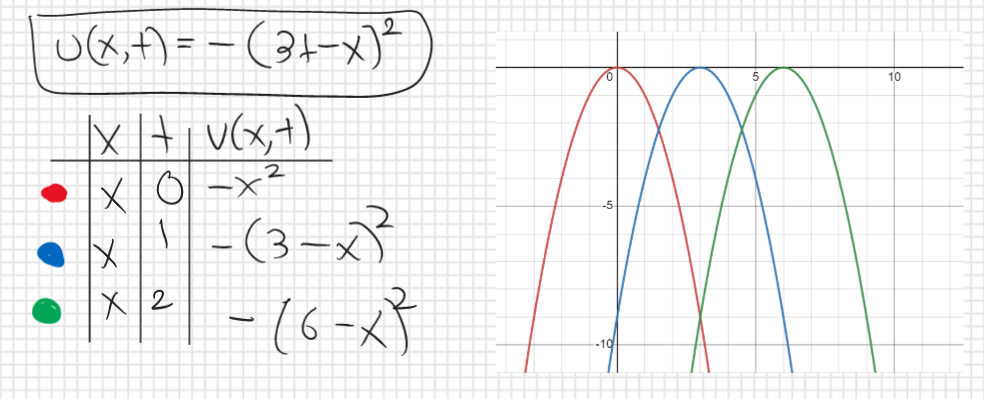
\includegraphics[width=\textwidth]{Images/transport.png}
\end{center}
\color{black}

\pagebreak 
\textbf{Problem 6:} Derive the transport equation $u_t + cu_x = 0$ using an approach similar to what we did for the heat equation in class. The notation is the same as in class, but this time assume that during the time interval from t to $t + \tau$ , all particles in an interval move to the nearest interval to their right, like in the figure below.
\color{blue}
\begin{enumerate}
    \item Let $u = u(x, t)$ measure the concentration of particles at x and t
    \item Let $h = \Delta x$
    \item Note that the number of particles on an interval of the rod of length h is roughly $hu(x, t)$
    \item Divide the rod into intervals of length h 
    \item Note the main assumption that with each time interval $[t, t + \tau]$, each particle moves from their position $x_i$ to $x_i + h$
    \item Thus, the number of particles at a given position $x$ at time $t + \tau$ will be 
    \[hu(x, t + \tau) = hu(x, t) + \delta\]
    where $\delta$ is a quantity representing the change in the number of particles at that point during that time step
    \item Finding delta:
    \[\delta = \text{in - out} = hu(x - h, t) - hu(x, t)\]
    \item So, 
    \[hu(x, t + \tau) = hu(x, t) + hu(x - h, t) - hu(x, t) \]
    \item Rearranging for the limit form:
    \[hu(x, t + \tau) - hu(x, t) = hu(x - h, t) - hu(x, t) \]
    \[u(x, t + \tau) - u(x, t) = h\left(\frac{u(x - h, t) - hu(x, t)}{h}\right)\]
    \[\frac{u(x, t + \tau) - u(x, t)}{\tau} = \frac{h}{\tau}\left(\frac{u(x - h, t) - hu(x, t)}{h}\right)\]
    \item Taking the limits:
    \[\lim_{\tau \to 0} \frac{u(x, t + \tau) - u(x, t)}{\tau} = u_t\]
    \[\lim_{h\to 0} \frac{u(x - h, t) - hu(x, t)}{h} = -u_x\]
    \item Combining:
    \[u_t = -\frac{h}{\tau}u_x\]
    \item Then, setting the constant $c := \frac{h}{\tau}$, 
    \[\ans{$u_t + cu_x = 0$}\]
    
\end{enumerate}

\end{document}